\documentclass[11pt]{article}
\usepackage[margin=1in]{geometry}
\usepackage{graphicx}
\usepackage{booktabs}
\usepackage{enumitem}
\usepackage{tikz}
\usepackage{fancyvrb}
\setlist{nosep,leftmargin=*}
\DefineVerbatimEnvironment{trans}{Verbatim}{fontsize=\scriptsize,frame=single,framesep=3pt}

\begin{document}

% ---------- Title page ----------
\begin{titlepage}
  \centering
  \vspace*{2cm}
  
\includegraphics[width=0.55\textwidth]{Logo.png}\\[1.5cm]
  {\large Department of Computer Science}\\[0.3em]
  {\large COMP438 --- Distributed Computing}\\[1.5cm]
  \rule{\linewidth}{0.4pt}\\[0.5em]
  {\LARGE\bfseries Peer-to-Peer Chat with a Directory Server}\\[0.4em]
  {\large Course Project --- Phase 1}\\[0.5em]
  \rule{\linewidth}{0.4pt}\\[2cm]
  {\large
  \begin{tabular}{ll}
    Baraa Rjoob        & 1221076 \\[0.3em]
    Abdallah Alqasrawi & 1221432 \\
  \end{tabular}}\\[2cm]
  {\large Instructor: Dr. Mohammad Helal}
  \vfill
\end{titlepage}

\section{Design}
The system has two programs. The \textbf{Directory} is a rendezvous server: it
tracks which clients are alive and brokers their network credentials, but it
never carries chat traffic. Each \textbf{Client} keeps one control connection to
the Directory and opens \emph{direct} TCP connections to other clients for chat.

On startup a client (i) connects to the Directory, (ii) opens its own listening
socket on an OS-assigned port for incoming peers, and (iii) sends an
\texttt{ALIVE} message every second carrying its id and that peer port. The
Directory records each client's IP, peer port, and last-seen time, and pushes
the list of active client ids to every client once per second. To chat, a client
asks the Directory for a target's IP and port, then connects to it directly.

\textbf{Rationale.} Messages are newline-delimited JSON because it is
self-describing and trivial to frame; a thread-per-connection model keeps the
code simple and lets the UI thread run without blocking on I/O; routing chat
\emph{directly} between peers keeps the Directory lightweight and removes it as a
traffic bottleneck. Usage:
\texttt{python3 directory.py [port]} and
\texttt{python3 client.py <id> [host] [port]}.

\section{Sockets and Concurrency}
\textbf{Socket count.}
\begin{itemize}
  \item \emph{Directory:} 1 listening socket, plus 1 control socket per connected client.
  \item \emph{Client:} 1 control socket to the Directory, 1 listening socket for
        incoming peers, and 1 socket per active peer chat.
\end{itemize}

\textbf{Concurrency.} Both programs use a thread-per-connection model.
\begin{itemize}
  \item The Directory accepts each control connection in its own handler thread,
        plus two background threads: a broadcaster (sends the active list) and a
        reaper (drops clients that stop sending \texttt{ALIVE}, i.e.\ soft state).
  \item Each client runs concurrent threads for the heartbeat, the Directory
        listener, the peer acceptor, and one reader per connected peer, so the
        input loop never blocks on the network.
  \item Shared registries (the Directory's presence/connection tables, the
        client's peer table) are guarded by a mutex. Writes to each socket are
        serialized by a per-socket lock so concurrent threads cannot interleave
        bytes from two frames on the same connection.
  \item On disconnect, the reader thread removes the peer and clears chat focus;
        the Directory's reaper removes any client silent beyond the timeout.
\end{itemize}

\textbf{Timing parameters.}

\begin{center}
\begin{tabular}{@{}lll@{}}
\toprule
\textbf{Parameter} & \textbf{Value} & \textbf{Meaning} \\
\midrule
Heartbeat interval & 1\,s & client $\to$ Directory \texttt{ALIVE} period \\
List broadcast     & 1\,s & Directory $\to$ clients active-list period \\
Alive timeout      & 3\,s & silence after which a client is reaped \\
\bottomrule
\end{tabular}
\end{center}
\noindent A client therefore disappears from every active list within roughly
3--4\,s of going silent.

\section{Establishing a Client-to-Client Connection}
\begin{enumerate}
  \item Client A issues \texttt{/chat B}, sending \texttt{CONNECT\_REQ\{dst:B\}}
        to the Directory.
  \item The Directory looks up B's record and replies with
        \texttt{PEER\_INFO\{ip, port\}} (or \texttt{ERROR} if B is unknown/inactive).
  \item A opens a direct TCP connection to B's advertised IP:port and sends
        \texttt{HELLO\{src:A\}} as its first frame, so B learns who connected.
  \item Both sides then exchange \texttt{CHAT} messages directly, with no further
        Directory involvement.
\end{enumerate}
If both clients request each other at the same time, two connections may form;
the first one registered is kept and the redundant socket is closed, so a pair
of clients shares exactly one direct connection.

\begin{center}
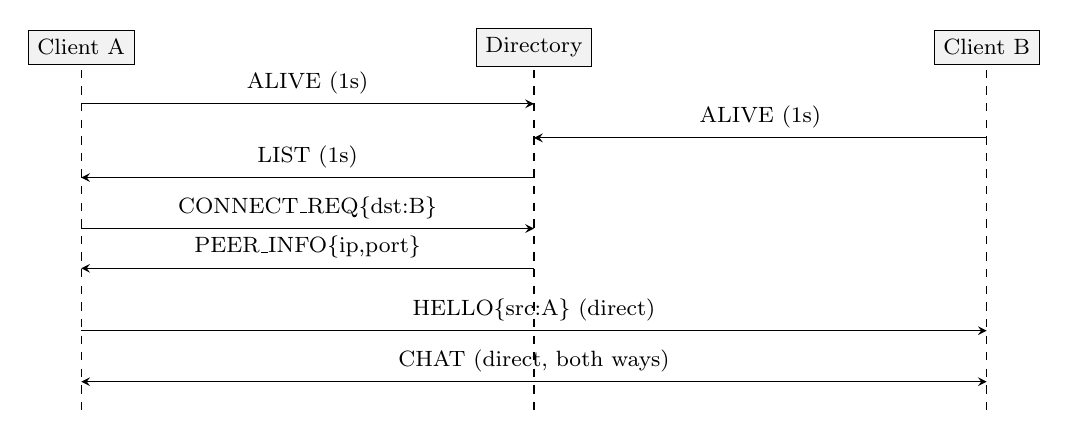
\begin{tikzpicture}[font=\footnotesize,>=stealth,xscale=1.15,yscale=0.72]
  % lifelines
  \node[draw,fill=gray!10] (A) at (0,0) {Client A};
  \node[draw,fill=gray!10] (D) at (5,0) {Directory};
  \node[draw,fill=gray!10] (B) at (10,0){Client B};
  \foreach \x in {0,5,10} \draw[dashed] (\x,-0.4) -- (\x,-6.4);
  % control-plane exchanges
  \draw[->] (0,-1.0)  -- node[above,sloped]{ALIVE (1s)}            (5,-1.0);
  \draw[->] (10,-1.6) -- node[above,sloped]{ALIVE (1s)}            (5,-1.6);
  \draw[->] (5,-2.3)  -- node[above,sloped]{LIST (1s)}             (0,-2.3);
  \draw[->] (0,-3.2)  -- node[above,sloped]{CONNECT\_REQ\{dst:B\}} (5,-3.2);
  \draw[->] (5,-3.9)  -- node[above,sloped]{PEER\_INFO\{ip,port\}} (0,-3.9);
  % data plane (direct, bypasses Directory)
  \draw[->] (0,-5.0)  -- node[above]{HELLO\{src:A\} (direct)}      (10,-5.0);
  \draw[<->](0,-5.9)  -- node[above]{CHAT (direct, both ways)}     (10,-5.9);
\end{tikzpicture}
\end{center}

\section{Application-Layer Header}
Every message is one JSON object terminated by a newline (\texttt{\textbackslash n}).
Newline framing is unambiguous because JSON encoding escapes any newline inside a
string, so a literal \texttt{\textbackslash n} never appears within a frame. The
mandatory \texttt{type} field acts as the header that selects how the remaining
fields are interpreted.

\begin{center}
\begin{tabular}{@{}llll@{}}
\toprule
\textbf{type} & \textbf{Direction} & \textbf{Fields} & \textbf{Purpose} \\
\midrule
\texttt{ALIVE}       & client $\to$ dir  & \texttt{src, peer\_port}     & heartbeat + register \\
\texttt{LIST}        & dir $\to$ client  & \texttt{clients[]}           & active ids (names only) \\
\texttt{CONNECT\_REQ}& client $\to$ dir  & \texttt{src, dst}            & request a peer's address \\
\texttt{PEER\_INFO}  & dir $\to$ client  & \texttt{dst, ip, port}       & peer's IP and port \\
\texttt{ERROR}       & dir $\to$ client  & \texttt{reason}              & target unknown/inactive \\
\texttt{HELLO}       & client $\to$ peer & \texttt{src}                 & identify on a new peer link \\
\texttt{CHAT}        & client $\to$ peer & \texttt{src, text}           & chat message \\
\bottomrule
\end{tabular}
\end{center}

\section{Sample Run}
Three processes on one host: one Directory and two clients, \texttt{alice} and
\texttt{bob}. Both register and heartbeat; \texttt{alice} lists the active
clients, opens a direct chat to \texttt{bob}, sends a message, then quits.

\noindent\textbf{Directory}
\begin{trans}
[directory] listening on 0.0.0.0:5071
[directory] registered 'bob' at 127.0.0.1:41437
[directory] registered 'alice' at 127.0.0.1:34223
[directory] alice -> connect info for bob
[directory] 'bob' disconnected
[directory] 'alice' disconnected
\end{trans}

\noindent\textbf{Client \texttt{alice}}
\begin{trans}
[client] 'alice' control->127.0.0.1:5071  peer-listen port=34223
Commands: /list  /chat <id>  /quit
> Active clients: alice, bob
> /chat bob
[connected] now chatting with 'bob'
> hello bob
> /quit
[disconnected] 'bob' left the chat
[client] bye
\end{trans}

\noindent\textbf{Client \texttt{bob}}
\begin{trans}
[client] 'bob' control->127.0.0.1:5071  peer-listen port=41437
Commands: /list  /chat <id>  /quit
[connected] 'alice' connected to you
[alice] hello bob
[client] bye
\end{trans}

\end{document}
